\documentclass[journal=jacsat,manuscript=article]{achemso}
\usepackage{paper_style}

%\usepackage{lipsum}  %% Package to create dummy text (comment or erase before start)

%% ===============================================
%% Setting the line spacing (3 options: only pick one)
\doublespacing
% \singlespacing
%\onehalfspacing
%% ===============================================


% %%%%%%%%%%%%%%%%%%%%%%%%%%%%%%%%%%%%%%%%%%%%%%%%%%%%%%%%%%
% SET THE TITLE
% %%%%%%%%%%%%%%%%%%%%%%%%%%%%%%%%%%%%%%%%%%%%%%%%%%%%%%%%%%

% TITLE:
\title{
First-Principles Studies of Substituent Effect on Squaraine Dyes\\
}

% AUTHORS:
\author{German Barcenas}
\affiliation{Boise State University}
\email{germanbarcenas@u.boisestate.edu}
\author{Austin Biaggne}
\affiliation{Boise State University}
\author{Kimo Wilson}
\affiliation{Boise State University}
\author{Bill Knowlton}
\affiliation{Boise State University}
\author{Bernard Yurke}
\affiliation{Boise State University}
\author{Lan Li}
\affiliation{Boise State University}





\begin{document}

\maketitle
% %%%%%%%%%%%%%%%%%%%%%%%%%%%%%%%%%%%%%%%%%%%%%%%%%%%%%%%%%%
% %%%%%%%%%%%%%%%%%%%%%%%%%%%%%%%%%%%%%%%%%%%%%%%%%%%%%%%%%%
% BODY OF THE DOCUMENT
% %%%%%%%%%%%%%%%%%%%%%%%%%%%%%%%%%%%%%%%%%%%%%%%%%%%%%%%%%%
% %%%%%%%%%%%%%%%%%%%%%%%%%%%%%%%%%%%%%%%%%%%%%%%%%%%%%%%%%%

% --------------------
\section{Introduction}
% --------------------
Employing DNA self-assembly methods is shown to enable the manipulation and mediation of chromophore dyes and give rise to Frenkel exciton delocalization among dimer systems\cite{Cannon2018LargeAggregates}. The study of monomers can lend insight into suitable candidates for more highly tuned dimer systems. Squaraine dyes in particular are reported to have spectral properties that make them a strong candidate to be used in conjunction with DNA nanotechnology\cite{Markova2013ComparisonLabels}⁠. This application of squaraines offers an opportunity to implement multichromophoric aggregate systems. 
By utilizing DNA as a scaffold for squaraine aggregation, dipole-dipole coupling occurs\cite{Cannon2017CoherentSystem}. This interatomic interaction model was first described by Kasha to allow the mixing of wavefunctions to access nondegenerate states\cite{Kasha1965TheSpectroscopy}. The splitting of energy levels results in new excited state behavior in aggregates as a bathochromic shift in absorbance (often referred as an J aggregate) or a hypsochromic shift (often referred to as an H aggregate)\cite{Wurthner2011J-aggregates:Materials} in conjunction with an observed splitting of the absorption peak known as Davydov splitting\cite{Zhong2019DavydovDimers}. The optical properties of these aggregates results in Frenkel excitons with coupling strengths related to these newly accessible states. 
To begin the study of a dye monomer to establish a baseline of multicomponent systems. Although aggregates are defined by their interaction distances, monomer electronic information is necessary when treating these interactions with point dipole approximations\cite{Abramavicius2009ExtractingSpectra}. Examples of other fields in which squaraines are being applied include organic photovoltaics\citep{Wei2012FunctionalizedPhotovoltaics, Chen2018DensityCell}, near infrared medical imaging\cite{Strassel2018SquaraineNm}⁠, and molecular photoswitches\citep{Kellis2019AnPhases, Scholes2011LessonsHarvesting} .

Squaraine dyes are composed of a squaric acid center. This central feature is a made from an electron-deficient aromatic group. This group is then combined with accepting of electron-rich groups, often in a symmetric manner by means of a methine bridge\cite{Ilina2020SquaraineChallenges}⁠. In this study, the electron-rich groups are trimethylindolenine with varied substitutes.

Previous work\cite{Bassal2017ExploringADC2}⁠ highlights the history of computational studies of squaraine dye studies. This work presents a smaller variation in squaraine dyes by maintaining the basic chemistry and only altering substituent groups. Squaraine dyes, unlike similar NIR cyanine dyes, are not symmetric and so from the monomer perspective have a potential for conformers to influence bulk spectral properties\cite{Kolosova2018MolecularSquaraines}. Highlighting squaraine conformer properties has recently become of interest due to the conformations potential to alter the final photophysical properties in squaraine applications\citep{Paterno2018ExcitedScenario}. Conformers investigated in this paper are : trans,syn or $C_{s}$ symmetry; cis,syn or $C_{2v}$ symmetry; and trans,anti or $C_{2h}$ symmetry.

This work investigates the ground state and excited state molecular structure of three conformations: trans,syn; cis,syn, and trans,anti for SQ-H2,SQ-Cl2 ,SQ-Cl1 and SQ-(CH3)2 otherwise referred to as SQ1, SQ4, SQ8 and SQ14 using density functional theory (DFT). This work presents a study of SQ1, SQ4, SQ8, and SQ14, in which substituents are changed according to their name. Investigations into the ground state and excited state electronic structures of these chromophores will enable a comparison of different substituents and their effects on electronic transition states necessary for the optimization of multichromophoric systems while also considering absorption properties.  


\begin{figure}[h]
\begin{subfigure}{.45\textwidth}
    \centering
    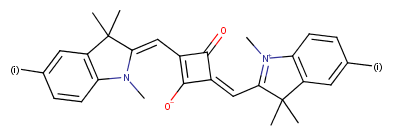
\includegraphics[width=.8\linewidth]{figures/SQi.png}
    \caption{}
\end{subfigure}
\begin{subfigure}{.45\textwidth}
    \centering
    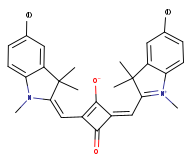
\includegraphics[width=.5\linewidth]{figures/sqi-cis.png}
    \caption{}
\end{subfigure}
\begin{subfigure}{.65\textwidth}
    \centering
    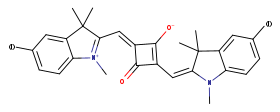
\includegraphics[width=.5\linewidth]{figures/sqi-trans.png}
    \caption{}
\end{subfigure}
    \caption{SQ-(i), where (i) sites represent substituent locations. SQ-H2, or SQ1 refers to squaraine derivative with (i) as H.Sq-Cl2, or SQ4 refers to squaraine derivative with (i) as Cl.SQ-Cl1, or SQ8 refers to squaraine derivative with (i) as Cl and H. SQ(CH3)2, or SQ14 referring to squaraine derivative with (i) as CH4. (a) shows the trans,anti conformation. (b) shows the cis,syn conformation. (c) shows the trans,syn conformation
}
    \label{fig:SQ dye}
\end{figure}


% --------------------
\section{Methodology}
% --------------------
The Gaussian 16 software package\cite{g16}⁠ was used in density functional density (DFT) calculations. Molecules were built and initially relaxed using the molecular editing software Avogadro\cite{Hanwell2012Avogadro:Platform}⁠ using the UFF\cite{Rappe1992UFFSimulations}⁠ method. All calculations were performed using the 6-31G+(d,p) basis set with the M06-2X\cite{Zhao2008TheFunction}⁠ correlation functional as previous works have shown a strong agreement with experimental results when compared with physical systems\citep{Jacquemin2016Excited-StateCC2,Jacquemin20150-0Compounds}. These structures were optimized using a tight root mean square residual force of $1*(10)^{-5}$  Hartree$\backslash$Bohr and an ultra fine integration grid of $99$ radial shells and $590$ angular points per shell. The use of tight root mean squared and ultra fine integration grid is recommended for optimizing larger molecules with soft frequency modes such as methyl groups\cite{AzaisTestingSuper-Resolution}. Ground state optimization of these molecules were verified to be optimized via ground state frequency checks to ensure no imaginary frequencies were present.

The optimized ground state structures were then used as the input geometry for excited state optimization calculations using time-dependent DFT (TD-DFT). The calculated excited state geometry was used to calculate the excited state frequency to ensure an optimized structure was achieved. Following this procedure was done to produce the 0-0 energy by implicitly including the zero-point vibrational energies\cite{Adamo2013TheTheory}. The ground state and excited state frequencies were then used to produce an absorption spectrum for each molecule and conformer. These spectra were generated using the general Frank-Condon (FC) method. From the ground state and excited state structures, parameters such as a dipole moment are accessible. A difference dipole,$\Delta d$, is calculated by taking the vector difference of the excited state and ground state dipole. The solvation energy, $\Delta G$ was calculated by taking the diference in ground state energies from a dye calcualted using SMD\cite{Marenich2009UniversalTensions} water and vacuum.

Conformation of squaraine dyes are referred here as trans,syn; cis,syn and trans,anti. In the study of monomers, it has been reported that there is a potential for coexistence of conformers in solution with conformation being substituent sensitive\citep{Kolosova2019MolecularSquaraines,Rohr2018ExcitonDimers}⁠. The population percentages were investigated using the Boltzmann distribution.
The difference dipole 


Experimental discussion? Talk to Kimo

\section{Results}
When comparing the results of conformer to experimental conditions and Boltzmann population distributions, the trans,anti conformation is the most dominate population and is closest to the experimental peak absorbance. All spectra exhibit a weak vibronic shoulder followed by a strong absorption peak in the orange wavelength region. This is narrow band with shoulder has been reported in previous literature of squaraine absorption bands \citep{Qin2013ACells,Zheng2015ContributionDevices,Yang2017ThePerformance,Borrelli2014TheoreticalDye,Kuster2015CoupledPendulums,Brixner2017ExcitonSystems}. The trans,syn conformation had a negligible Boltzmann population of $<5\%$ and so this shoulder should not effect a bulk absorption spectra in solution. This follows with conclusions by others in that, for squaraine with a mirror symmetry, trans,anti dominates the the population with a non-negligible percentage also of cis,syn symmetry\cite{Borrelli2014TheoreticalDye}. In fact, the cis,syn conformation has been shown to be the more energetically favorable conformer by adding a dicyanovinyl substituent to the squaric moiety\cite{Qin2013ACells}.  


\begin{figure}[h]
    \centering
    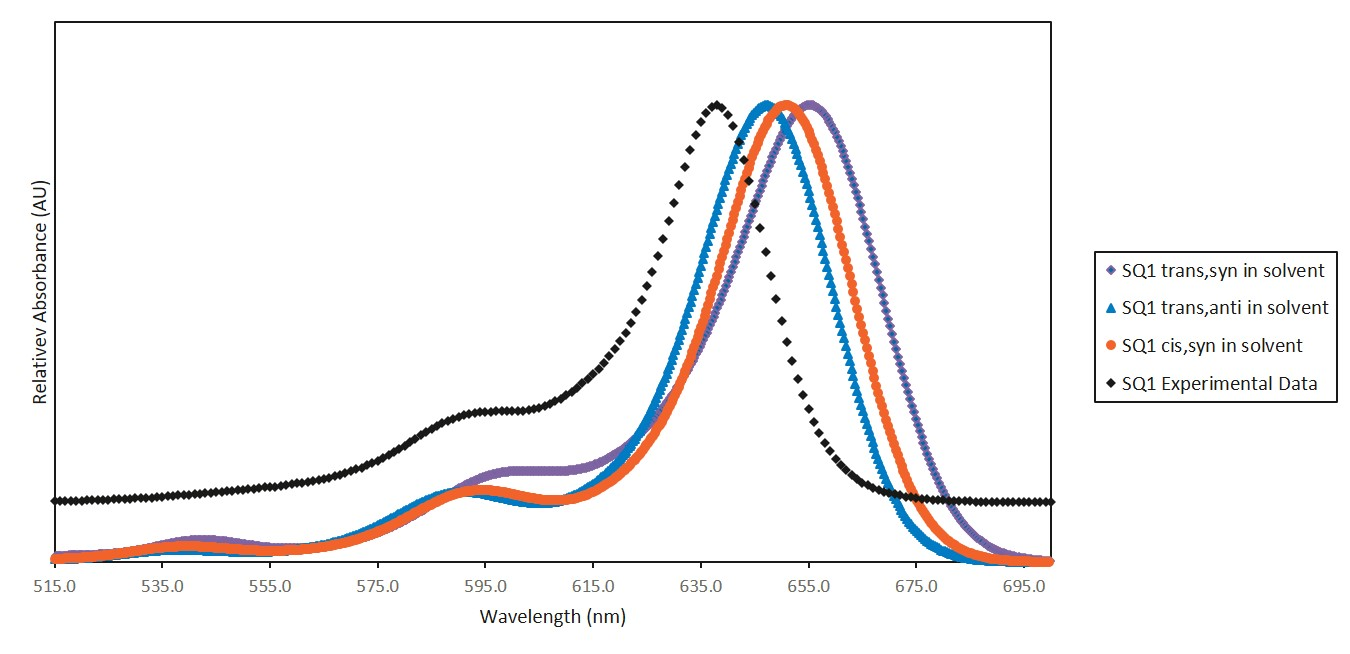
\includegraphics[width=16cm,height=8cm]{figures/sq1_conformer_exp.jpg}
    \caption{Comparison of SQ1 conformer spectra generated using FC approximation in IEFPCM water solvent. All structures were optimized  using 6-31+G(d,p) basis set and M06-2X exchange correlation functional.}
    \label{fig:SQ1 conformers}
\end{figure}

When comparing SQ1 and SQ4 trans,anti, experimental results, and vacuum calculations, M06-2X in vacuum is able to predict the experimental absorption spectrum curve before the inclusion of a solvent. The inclusion of solvent is able to predict the peak of SQ1 within 1.4$\%$ 0r 0.03 $eV$ of experiment and SQ4 within 2.4$\%$ or 0.02 $eV$. A blue shift of 0.03 $eV$ is a well-known phenomena of TD-DFT calculations with this family of cyanine-type dyes\cite{Jacquemin2011Excited-stateEnvironments}. Although the absorption peaks are not exact, the absorption curves are of a similar shape. This matching of shapes suggests that excited state calculations are capable of predicting the excited state geometry accurately. 

A popular classification and quantification of substituents as electron donating and accepting is known as the Hammet parameter\cite{Hansch1991AParameters}. In this scheme,$\sigma_{p}^{+}$ is a parameter associated with substituents that interact with strong resonance reaction systems (+ superscript) as a general correction to the $\sigma_{p}$ parameter which does not take this approach. The chlorine substituent in SQ4 acts as a electron donating addition and is capable of delocalizing a positive charge according to the Hammet parameter. This electron localization manifest itself when comparing dipole moments, since dipole moments of a symmetric dye such as a squaraine should result in the an electronic structure with a more positive aromatic group relative to the electron-deficient squaric moiety. This substituent leaves the absorption relatively undisturbed due to the relatively uncharged $\pi$ conjugation length of the dye\cite{Punitharasu2019-ExtendedResponse}.


\begin{figure}[h]
    \centering
    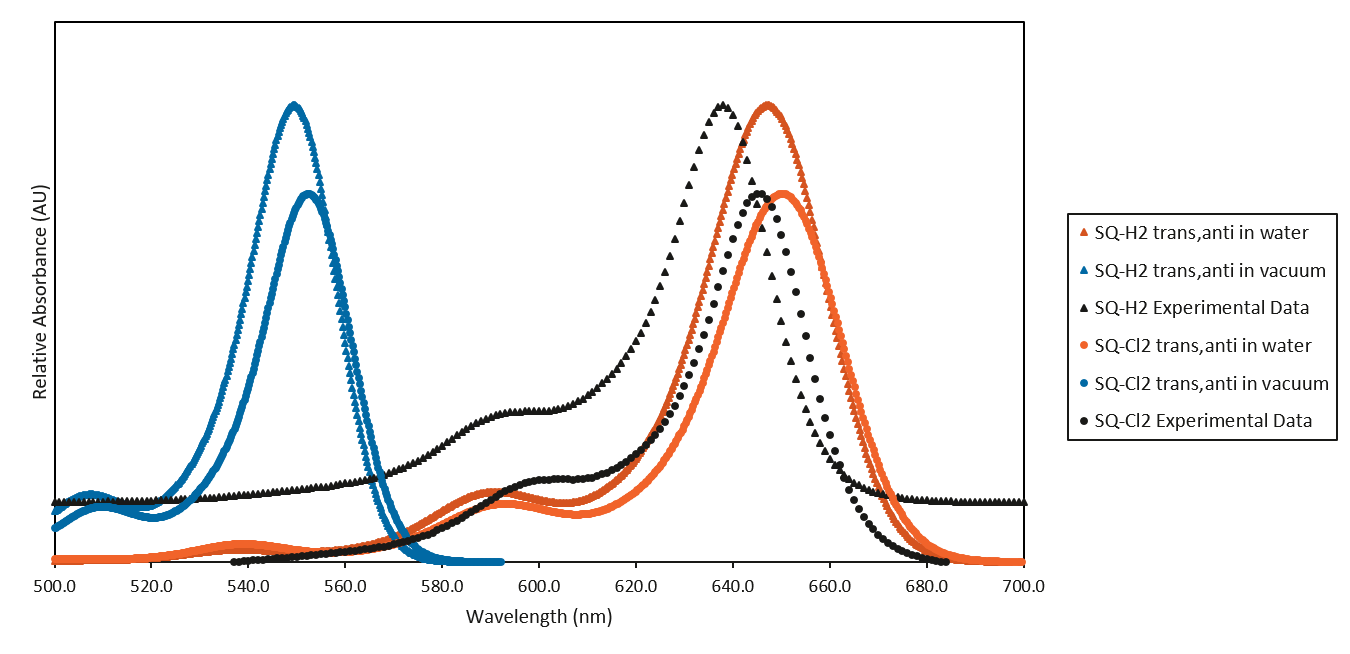
\includegraphics[width=15cm,height=8cm]{figures/sq1-sq4.png}
    \caption{Comparison of  SQ1 and SQ4 spectra generated using FC approximation in vacuum, IEFPCM water solvent, and experimental data. All structures were optimized using 6-31+G(d,p) basis set and M06-2X exchange correlation functional.}
    \label{fig:SQ1 and SQ4}
\end{figure}


\begin{figure}[h]
    \centering
    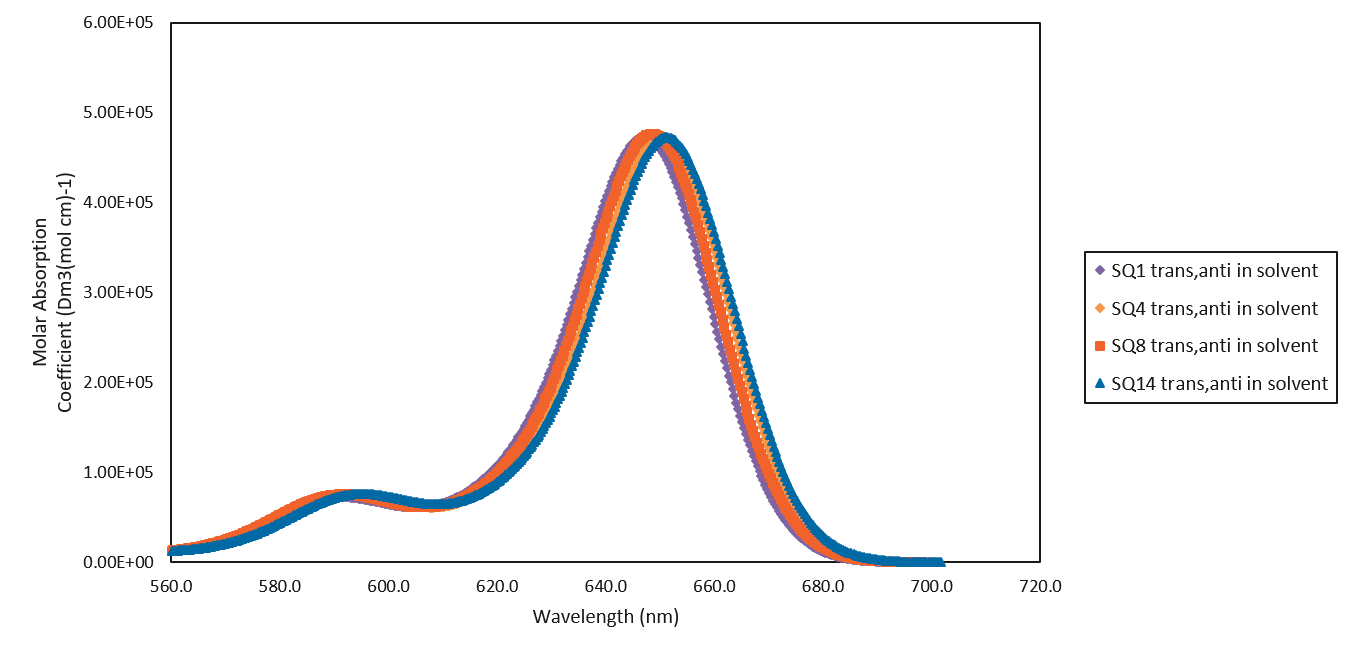
\includegraphics[width=15cm,height=8cm]{figures/sq1_4_8_14.png}
    \caption{Comparison of  SQ1, SQ4, SQ8, and SQ14 trans,anti conformation spectra generated using FC approximation in IEFPCM water solvent. All structures were optimized  using 6-31+G(d,p) basis set and M06-2X exchange correlation functional.}
    \label{tab:SQ1,4,8,14 absorption}
\end{figure}


\begin{table}[h]
    \centering
    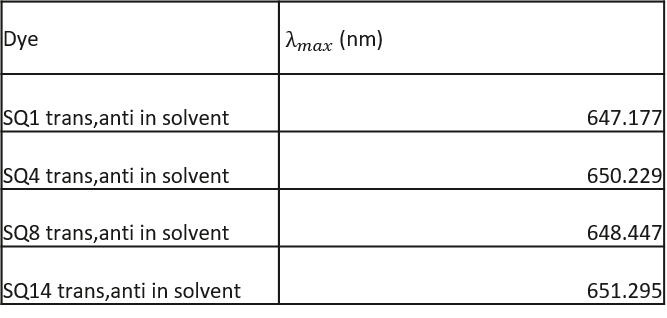
\includegraphics[width=17cm,height=5cm]{figures/sq1_4_8_14-table.png}
    \caption{Squaraine dye conformation electronic data. The Hammet parameter, $\sigma_{p}^{+}$\cite{Hansch1991AParameters}, GSDM is the ground state dipole moment in Debye, ESDM is the excited state dipole moment in Debye, Δd is the difference dipole calculated as the difference ESDM and GSDM in Debye, μ is the transition state dipole moment in Debye, S1-S0 is the 0-0 energy in eV, $\Delta G$ is the solvation energy in eV, and $\lambda_{max}$ is the wavelength associated with the peak in absorption spectrum generated using the Frank Condon approximation . All calculations were done using the 6-31G+(d,p) basis set and M06-2X exchange correlation function. All electronic data was calculated using water IEFPCM. Solvation energy was calculated using water SMD.}
    \label{tab:SQ1,4,8,14 lambda data}
\end{table}


\newpage
The altering of substituents of trimethylindolenine squaraine dyes does not significantly alter the peak absorption of these dyes. This behavior suggests absorption properties are more sensitivity to $\pi$ conjugation lengths\cite{Yamaguchi2008HowEfficiency}.  Meanwhile, these substituents allow for an opportunity to change the electronic properties of dyes. When comparing trans,anti $C_{2h}$ data in Table \ref{tab:SQ1,4,8,14 lambda data}, the molecule with a break in symmetry, SQ8, exhibits a $\Delta d$ relative to the symmetric SQ1, SQ4, and SQ14. Meanwhile, when comparing $\mu$ of SQ4, SQ8, and SQ14, they remain relatively unperturbed. 
When building a system meant for aggregation, these substituents can also effect the aggregation behavior. The difference between SQ4 and SQ14 are related to the solvation energy.

When comparing the cis,syn $C_{2v}$ data, there is now a dipole relative to the electronic structure of the dyes and so $\Delta d$ values become larger. This symmetry effect is less noticeable in SQ-Cl1 since this system already had broken mirror symmetry. In general, $\mu$ values for cis,syn fell. Conformation is known to impact $\mu$\cite{Brand2011HowStructure} and the small change in $\mu$ suggests a that the squaraine dye is polarized along the short axis as this axis is least effected by conformation changes\cite{Lopata2011Excited-stateTD-ZINDO}. $\lambda_{max}$ remains relatively similar but do increase by about 4nm from trans,anti to cis,syn. This is line with previous literature\cite{Borrelli2014TheoreticalDye}.
The inclusion of solution into the calculation can serve as a measure for likelihood of aggregation; more negative solvation energy is associated with a more thermdynamically favorable solution. For less negative solvation energy, dye aggregation is not as favorable. When comparing the solvation energy, SQ-Cl2 shows a higher likelihood to aggregate if we use solvation energy as a proxy for solubility\cite{Fothergill2018AbDyes}. 
\newpage
\newpage
\section{Discussion}

Although this squaraine dye has potential conformers, trans,anti with $C_{2h}$ symmetry is the dominate population. Cis,syn can be made to be the dominant conformation by adding a substituent to the squaric center. In general, trans,anti conformers have a negligible $\Delta d$ which can be attributed to symmetry of the dye.
The choice of substituents in this study do not extend the conjugation length and so the absorption peak remains relatively static. This leaves altering of electronic properties as an option without potentially compromising the narrow intense absorption that is characteristic of squaraine dyes.
In general, the substituents chosen all raise the squaraine $\mu$ to roughly 16$D$. The greater variability is in $\Delta d$.
As some application note, these systems are of interest due to dye aggregates, with stronger aggregation preferred to encourage dipole coupling for multichromophoric systems
\section{Conclusion}
Changing substituents allows for the changing of electronic properties while optical properties are help relatively constant. Trimethylindolenine squaraine dyes offer an opportunity for highly tuned dye applications. Chlorine substituents are an attractive choice for altering the electronic properties of squaraine dyes without altering the photophyiscal properties. Squaraine dyes with substituents bonded to the donating heterocycles should be expected to have a trans,anti conformation in solution. The addition of donating substituents to squaraine can alter the conjugation length of the dye and minutely effect the absorption maximum. Concomitantly, dipole and solvation energies are altered due to the change in polarity associated with 
% %%%%%%%%%%%%%%%%%%%%%%%%%%%%%%%%%%%%%%%%%%%%%%%%%%%%%%%%%%
% %%%%%%%%%%%%%%%%%%%%%%%%%%%%%%%%%%%%%%%%%%%%%%%%%%%%%%%%%%
% REFERENCES SECTION
% %%%%%%%%%%%%%%%%%%%%%%%%%%%%%%%%%%%%%%%%%%%%%%%%%%%%%%%%%%
% %%%%%%%%%%%%%%%%%%%%%%%%%%%%%%%%%%%%%%%%%%%%%%%%%%%%%%%%%%

\newpage
\bibliography{references.bib} 

% ==========================
% ==========================
% ==========================


\end{document}